%!TEX root = ../template.tex
%%%%%%%%%%%%%%%%%%%%%%%%%%%%%%%%%%%%%%%%%%%%%%%%%%%%%%%%%%%%%%%%%%%
%% chapter1.tex
%% NOVA thesis document file
%%
%% Chapter with introduction
%%%%%%%%%%%%%%%%%%%%%%%%%%%%%%%%%%%%%%%%%%%%%%%%%%%%%%%%%%%%%%%%%%%

\typeout{NT FILE chapter1.tex}%

\chapter{Introduction}
\label{cha:introduction}

\prependtographicspath{{Chapters/Figures/Covers/}}

% epigraph configuration
\epigraphfontsize{\small\itshape}
\setlength\epigraphwidth{12.5cm}
\setlength\epigraphrule{0pt}


\includegraphics[width=0.1\linewidth]{NOVAthesisFiles/Images/novathesis-insignia}\hfill

\includegraphics[width=0.875\linewidth]{NOVAthesisFiles/Images/novathesis-text}

\noindent This is the \gls{novathesis} \LaTeX\ template Version \novathesisversion\ from \novathesisdate.

\epigraph{
  This work is licensed under the \href{https://www.latex-project.org/lppl/lppl-1-3c/}{\LaTeX\ Project Public License v1.3c}.
  To view a copy of this license, visit the \href{https://www.latex-project.org/lppl/}{LaTeX project public license}.
}

\section{If You Use this Template…} 
\label{sub:if_you_use_this_template}

This first Chapter introduces the \gls{novathesis} template and how it is organized. In Chapter~\ref{cha:users_manual} you can find some specific instructions on how to use the \gls{novathesis} template.  Chapter~\ref{cha:a_short_latex_tutorial_with_examples} shows some examples and give some hints on how to write your text. Please read these next Chapters carefully.

\subsection{Your Time is Precious}
\label{sub:time_is_money}

Did you learn how to drive by sitting by the wheel and throwing your car into the road?  Most probably you did take your time \emph{learning the rules} and \emph{practicing} first! Likewise, it is not wise to throw yourself at the task of writing a thesis/dissertation in \LaTeX\ without seriously considering the following statement!


% subsection subsection_name (end)
% \begin{quote}
%   \rule{\linewidth}{2pt}
% If you are going to spend zillions of hours writing your thesis/dissertation using this \gls{novathesis} template, be wise and spend a couple of hours learning how to use it properly by reading this manual.  And then be even wiser and spend a few more hours \href{https://github.com/joaomlourenco/novathesis/wiki#learning-latex}{learning some \LaTeX}.  I am sure that the time you are investing now will pay itself countless times before you submit your thesis/dissertation.
% \hfill \raisebox{-1ex}{\itshape João Lourenço}\\[-1ex]
%   \rule{\linewidth}{2pt}
% \end{quote}
\bgroup
\renewcommand{\mkcitation}[1]{\\[0ex]\parbox{\linewidth}{\hfill\textbf{#1}}}
\blockquote[João Lourenço]{%
  \rule{\linewidth}{2pt}\\\itshape
  If you are going to spend zillions of hours writing your thesis/dissertation using this \gls{novathesis} template, be wise and spend a couple of hours learning how to use it properly by reading this manual.  And then, be even wiser, and spend a few more hours \href{https://github.com/joaomlourenco/novathesis/wiki\#learning-latex}{learning some \LaTeX}.  I am sure that the time you are investing now will pay itself countless times before you submit your thesis/dissertation.\\\nopagebreak
  % \hfill \raisebox{-1ex}{\itshape João Lourenço}\\[-1ex]
  \rule{\linewidth}{2pt}%
}
\egroup

\subsection{Recognition}
\label{sub:recognition}

The \gls{novathesis} tempalte was born in~1996, and what you see now accumulates to many many hundreds (thousands?!) of working hours, unpaid and stollen from family and friends.  This work is available to the community under the \href{LaTeX project public license}{\LaTeX\ Project Public License v1.3c}, which means you are entitled to use it for free.  However, if you decide to use this template to write your thesis/dissertation, \textbf{be fair to the developers} and:
\begin{enumerate}
  \item Cite the \gls{novathesis} manual~\cite{novathesis-manual} in a place of your choice (e.g., in the \emph{Acknowledgments}) of your thesis/disseration with “\verb!\cite{novathesis-manual}!” .  If you cite it this way, the correct entry will be added automatically to your bibliography (no need to worry with the necessary BibTeX entry, as it will be added automatically);
  \item Go to the
\href{https://github.com/joaomlourenco/novathesis}{project web page in GitGub} and give the project a star (marked with a red ellipse at the top-right in Figure~\ref{fig:github}); and
  \item Make a donation by visiting the \gls{novathesis} project page and clicking in the button marked with a green ellipse at the top-center in Figure~\ref{fig:github}).  Alternatively, just click \href{https://www.paypal.com/donate/?hosted_button_id=8WA8FRVMB78W8}{\fcolorbox{DarkGreen}{gray!15}{\textbf{~HERE~}}} and your browser will be directed to the right page.
\end{enumerate}

\begin{figure}[htbp]
  \centering
    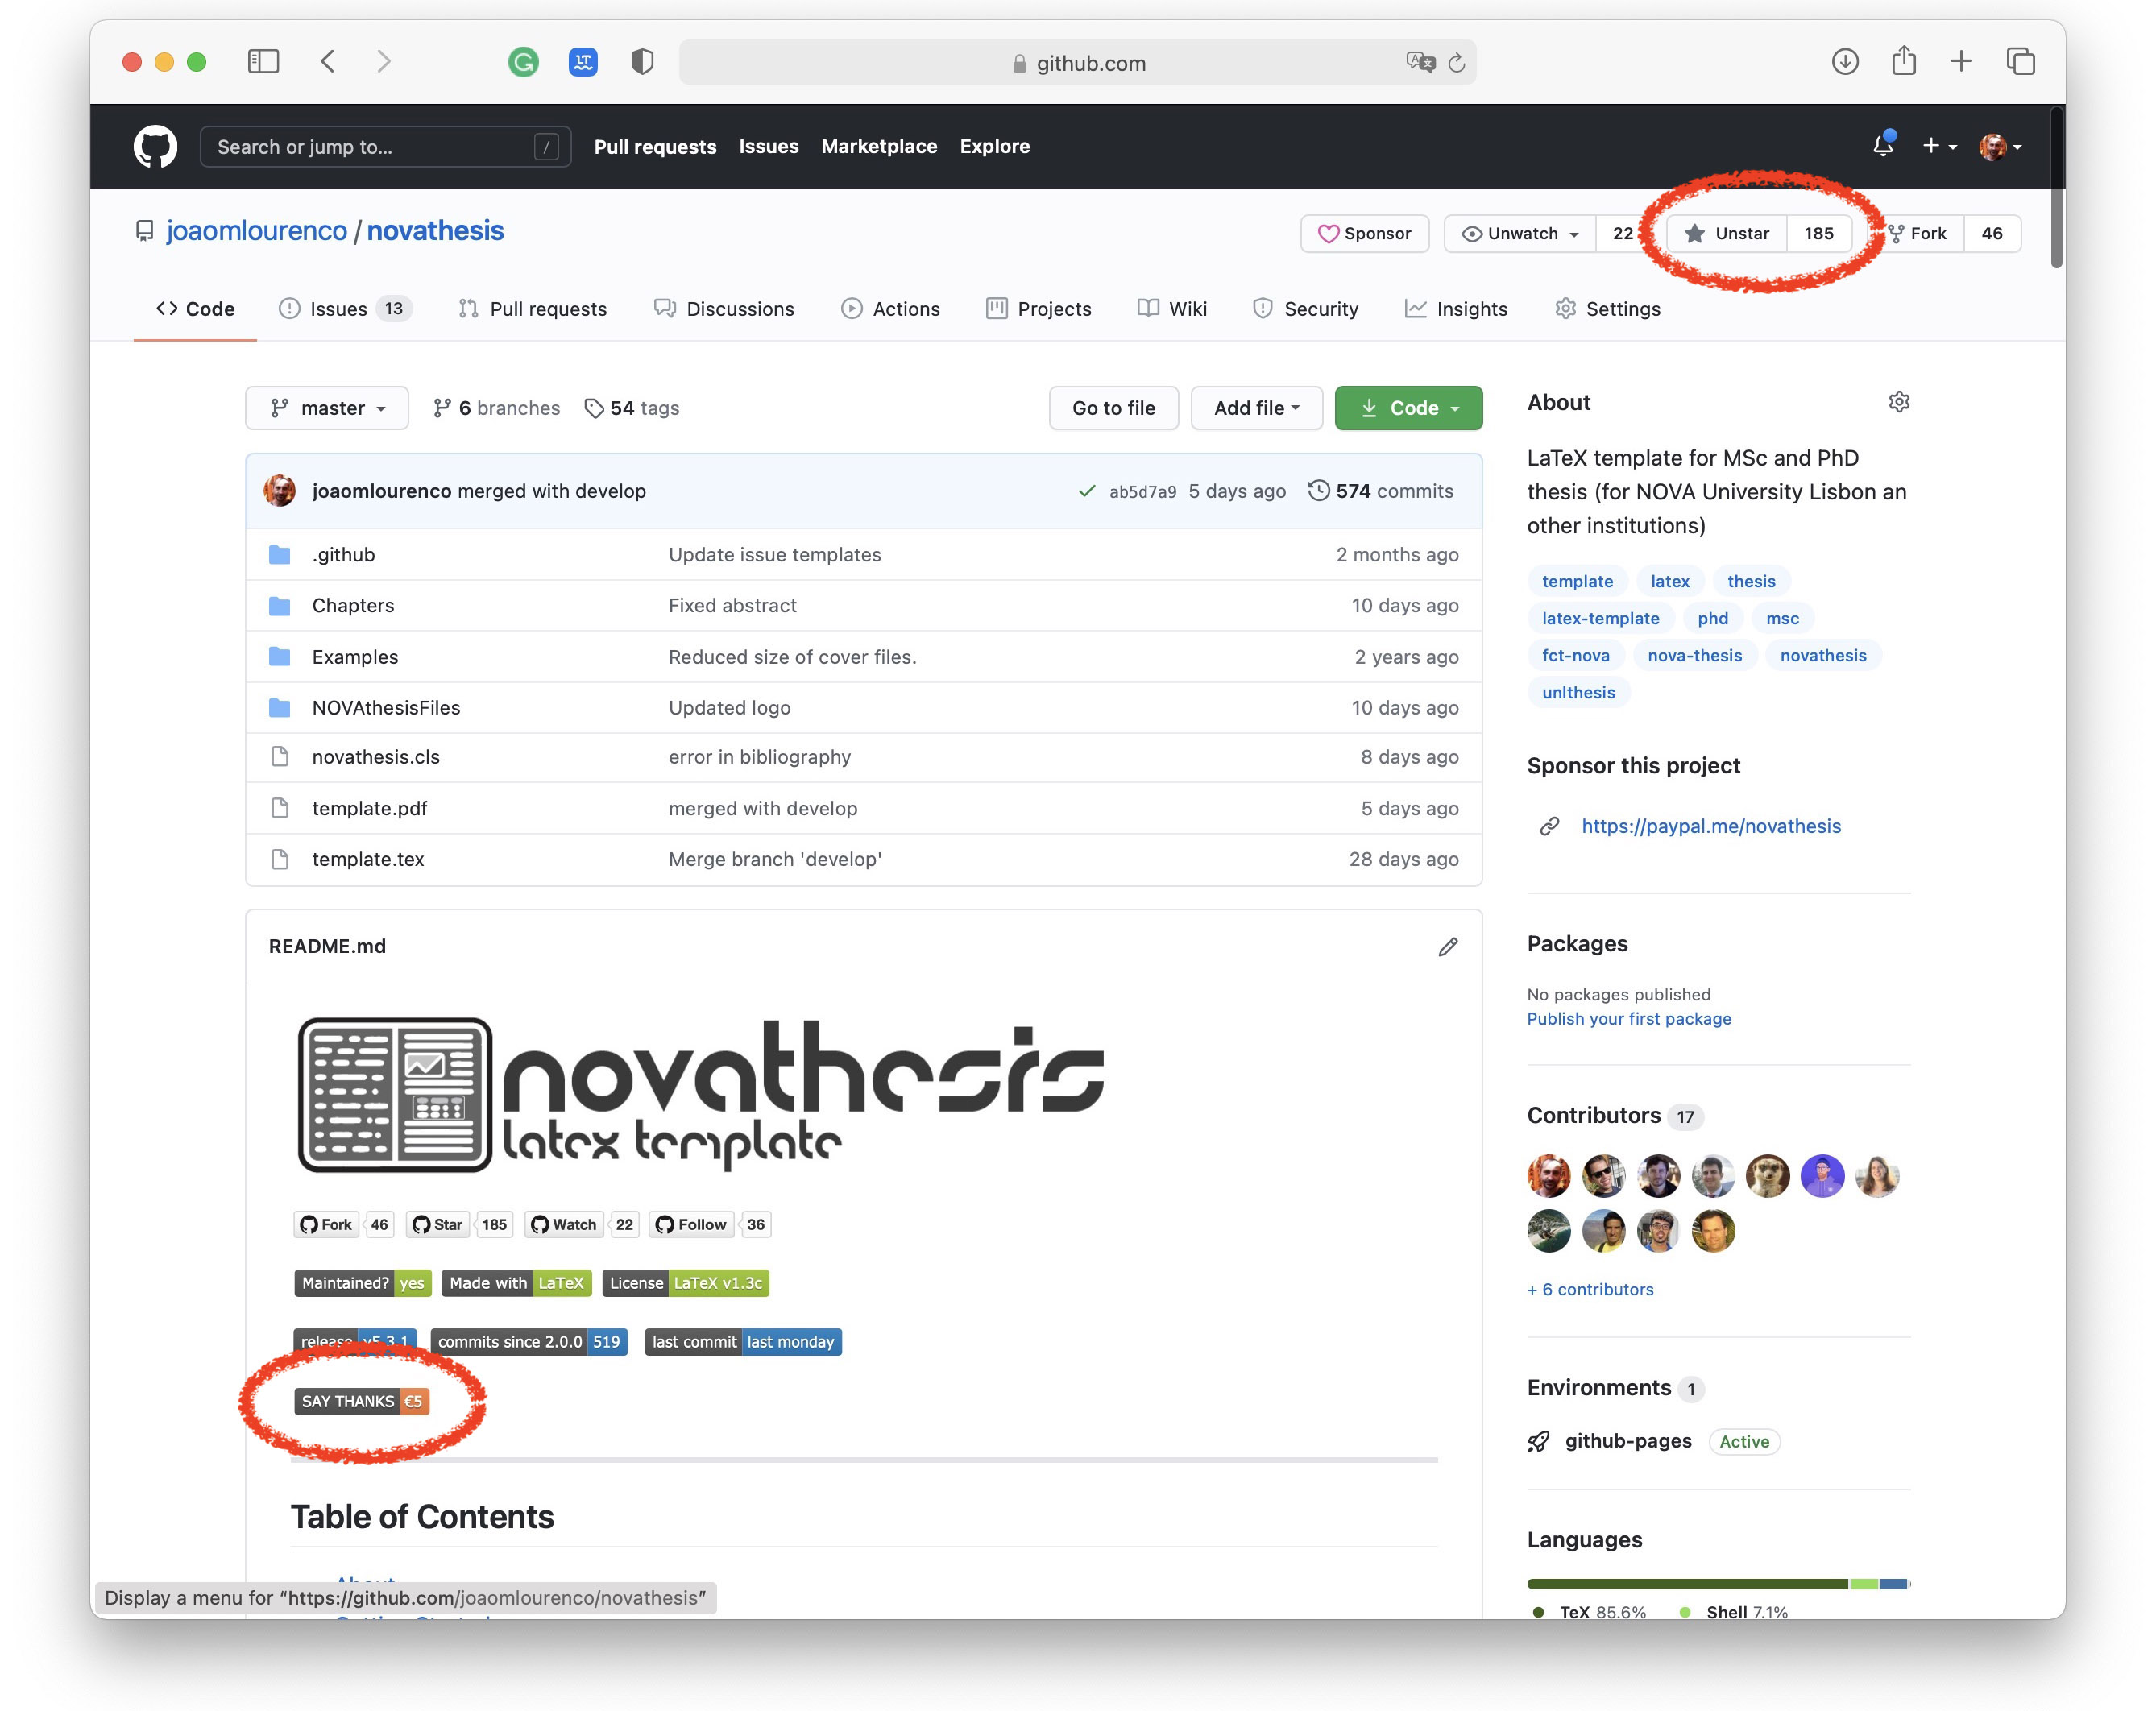
\includegraphics[width=0.7\textwidth]{github1}
  \caption{The \gls{novathesis} project web page in GitHub.}
  \label{fig:github}
\end{figure}

\section{The \emph{NOVAthesis} template}
\label{sec:a_bit_of_history}

% \newenvironment{ntUniversity}[1]{
%     \begin{longtblr}[
%         % presep = 1ex,
%         % postsep = 1ex,
%         caption = {#1's Schools supported by the \novathesis\ template.},
%         label = {tab:supported_schools_#1},
%         % label=none,
%     ]{colspec = {Q[c,m]X[j,m]},
%         rowhead = {1},
%         row{odd} = {GhostWhite},
%         % row{even} = {yellow},
%         row{1}  = {font=\bfseries, l, Schlgray, ht=1cm},
%     }
%         \toprule
%      ~ & #1 \\
%         \midrule
% }{%
%         \bottomrule
%     \end{longtblr}
% }


The \gls{novathesis} template was born at the \gls{DI} of  \gls{FCT} of \gls{NOVA}, Portugal.  But the user base grew… initially to other Departments of FCT-NOVA, then to other Schools of NOVA, and later to other Schools of other Universities.  Currently more than~25 Schools are natively supported by the \gls{novathesis} template (see Tables~\ref{tab:supported_schools_NOVA University Lisbon}, \ref{tab:supported_schools_University of Lisbon}, \ref{tab:supported_schools_University of Minho}, \ref{tab:supported_schools_Instituto Politécnico de Lisboa}, \ref{tab:supported_schools_Instituto Politécnico de Setúbal}, and \ref{tab:supported_schools_Other Universities/Schools/Degrees}).

\newenvironment{ntUniversity}[1]{
  \renewcommand\tabularxcolumn[1]{m{##1}}% for vertical centering text in X column
  % \renewcommand\cellgape{\Gape[1cm]}
  % \setcellgapes{20pt}
  % \makegapedcells
  % % \setlength{\extrarowheight}{20pt}
  % \renewcommand{\arraystretch}{2}
  \rowcolors{1}{}{GhostWhite}
    \xltabular{\linewidth}{cX}%
      \caption{#1's Schools supported by the \gls{novathesis} template\label{tab:supported_schools_#1}}\\
    \toprule%
    \rowcolor{Gainsboro}%
    & \Gape[1.5ex]{\thead[l]{#1}}\\
    \midrule%
}{%
    \bottomrule
    \endxltabular%
}

\makeatletter
\newtoggle{coverspace}
\newcommand{\docCover}[1]{%
  \setlength{\fboxsep}{0pt}%
  \togglefalse{coverspace}%
    \Gape[1.5ex]{\begin{mcellbox}[cc]
    \@for\i:=#1\do{%
      \fbox{\colorbox{White}{\includegraphics[align=c,width=1.5cm]{1up/\i}}}%
        \ifx\@xfor@nextelement\@nnil
          % last iteration
        \else
          % not last iteration
          \iftoggle{coverspace}{\togglefalse{coverspace}\\\\[-14pt]}{\toggletrue{coverspace}~}%
        \fi
  }%
    \end{mcellbox}}
}
\makeatother
\newcommand{\schlName}[3]{\textbf{#1} (\href{#3}{#2})}
\newcommand{\degreeName}[3]{\newline\null\quad • #1 \href{#3}{(#2)}}

\begin{ntUniversity}{NOVA University Lisbon}
  {
      \docCover{nova-fct-phd-en,nova-fct-msc-en}
  } &  {
    \schlName{NOVA School of Science and Technology}{FCT-NOVA}{https://www.fct.unl.pt}
    \degreeName{All PhD Programs}{PhD}{https://www.fct.unl.pt/en/education/phd-programmes}
    \degreeName{All MSc Programs}{MSc}{https://www.fct.unl.pt/en/education/master-degrees}
  }\\
  {
      \docCover{nova-fcsh-phd-en,nova-fcsh-msc-en}
  } &  {
    \schlName{NOVA School of Social Sciences and Humanities}{FCSH-NOVA}{https://www.fcsh.unl.pt}
    \degreeName{All PhD Programs}{PhD}{https://www.fcsh.unl.pt/cursos/\#doutoramentos}
    \degreeName{All MSc Programs}{MSc}{https://www.fcsh.unl.pt/cursos/\#mestrados}
  }\\
  {
      \docCover{nova-ims-phd-en,nova-ims-msc-mmaa-en,%
                nova-ims-msc-megi-en,nova-ims-msc-mgi-en,%
                nova-ims-msc-mcsig-en,nova-ims-msc-mgt-en}
  } &  {
    \schlName{NOVA Information Management School}{NOVA-IMS}{https://www.novaims.unl.pt}
    \degreeName{All PhD Programs}{PhD}{https://www.novaims.unl.pt}
    \degreeName{Master's in Data Science and Advanced Analytics}{MMAA}{https://www.novaims.unl.pt/mdsaa-ba}
    \degreeName{Master's in in Statistics and Information Management}{MEGI}{https://www.novaims.unl.pt}
    \degreeName{Master's in Information Management}{MGI}{https://www.novaims.unl.pt}
    \degreeName{Master's in Geographic Information Systems and Science}{MCSIG}{https://www.novaims.unl.pt/unigis}
    \degreeName{Master's in Geospatial Technologies}{GeoTech}{https://www.novaims.unl.pt/geotech}
  }\\
  {
      \docCover{nova-ensp-phd-en,nova-ensp-msc-en}
  } &  {
    \schlName{National School of Public Heath}{ENSP-NOVA}{https://www.ensp.unl.pt}
    \degreeName{All PhD Programs}{PhD}{https://www.ensp.unl.pt/courses/phds}
    \degreeName{All MSc Programs}{MSc}{https://www.ensp.unl.pt/courses/masters}
  }\\
  {
      \docCover{nova-itqb-phd-green-en,nova-itqb-msc-green-en,%
                nova-itqb-phd-gray-en,nova-itqb-msc-gray-en}
  } & {
    \schlName{Instituto de Tecnologia Química e Biológica}{ITQB-NOVA}{https://www.itqb.unl.pt}
    \degreeName{All PhD Programs}{PhD}{https://www.itqb.unl.pt/education/PhD\%20Programs}
    \degreeName{All MSc Programs}{MSc}{https://www.itqb.unl.pt/education/masters-courses}
  }\\
\end{ntUniversity}

\begin{ntUniversity}{University of Lisbon}
  {
    \docCover{ulisboa-ist-phd-en,ulisboa-ist-msc-en}
  } & {
    \schlName{Instituto Superior Técnico}{IST-UL}{https://tecnico.ulisboa.pt}
    \degreeName{All PhD Programs}{PhD}{https://tecnico.ulisboa.pt/en/education/courses/phd-programmes/}
    \degreeName{All MSc Programs}{MSc}{https://tecnico.ulisboa.pt/en/education/courses/masters-programmes}
  }\\
  {
    \docCover{ulisboa-fc-phd-en,ulisboa-fc-msc-en}
  } & {
    \schlName{Faculdade de Ciências}{FCUL}{https://ciencias.ulisboa.pt}
    \degreeName{All PhD Programs}{PhD}{https://ciencias.ulisboa.pt/en/educational-offer/}
    \degreeName{All MSc Programs}{MSc}{https://ciencias.ulisboa.pt/en/educational-offer/}
  }\\
  {
    \docCover{ulisboa-fmv-phd-en,ulisboa-fmv-msc-en}
  } & {
    \schlName{Faculdade de Medicina Veterinária}{FMV-UL}{https://www.fmv.ulisboa.pt}
    \degreeName{All PhD Programs}{PhD}{https://www.fmv.ulisboa.pt/en/study/phd}
    \degreeName{All MSc Programs}{MSc}{https://www.fmv.ulisboa.pt/pt/ensino/mestrados}
  }\\
\end{ntUniversity}


\newdata*{schlname}
\newdata*{schlurl}
\schlname(ea):={School of Architecture}
\schlurl(ea):={https://www.uminho.pt/EN/uminho/Units/schools-and-institutes/Pages/School-of-Architecture.aspx}
\schlname(ec):={School of Sciences}
\schlurl(ec):={https://www.uminho.pt/EN/uminho/Units/schools-and-institutes/Pages/school-of-sciences.aspx}
\schlname(ed):={School of Law}
\schlurl(ed):={https://www.uminho.pt/EN/uminho/Units/schools-and-institutes/Pages/school-of-law.aspx}
\schlname(ee):={School of Engineering}
\schlurl(ee):={https://www.uminho.pt/EN/uminho/Units/schools-and-institutes/Pages/school-of-Engineering.aspx}
\schlname(eeg):={School of Economics and Management}
\schlurl(eeg):={https://www.uminho.pt/EN/uminho/Units/schools-and-institutes/Pages/school-of-economics-and-management.aspx}
\schlname(em):={School of Medicine}
\schlurl(em):={https://www.uminho.pt/EN/uminho/Units/schools-and-institutes/Pages/school-of-Medicine.aspx}
\schlname(ep):={School of Psychology}
\schlurl(ep):={https://www.uminho.pt/EN/uminho/Units/schools-and-institutes/Pages/school-of-psychology.aspx}
\schlname(ese):={School of Nursing}
\schlurl(ese):={https://www.uminho.pt/EN/uminho/Units/schools-and-institutes/Pages/school-of-nursing.aspx}
\schlname(i3b):={Research Institute 13Bs}
\schlurl(i3b):={https://www.uminho.pt/EN/uminho/Units/schools-and-institutes/Pages/Institute-I3Bs.aspx}
\schlname(ics):={Institute of Social Sciences}
\schlurl(ics):={https://www.uminho.pt/EN/uminho/Units/schools-and-institutes/Pages/institute-of-social-sciences.aspx}
\schlname(ie):={Institute of Education}
\schlurl(ie):={https://www.uminho.pt/EN/uminho/Units/schools-and-institutes/Pages/institute-of-education.aspx}
\schlname(ilch):={School of Arts and Humanities}
\schlurl(ilch):={https://www.uminho.pt/EN/uminho/Units/schools-and-institutes/Pages/school-of-arts-and-humanities.aspx}

\begin{ntUniversity}{University of Minho}
    {
      \docCover{uminho-ea-phd-en,uminho-ea-msc-en}
    } & {
      \schlName{\theschlname(ea)}{\uppercase{ea}-UMINHO}{\theschlurl(ea)}
      \degreeName{All PhD Programs}{PhD}{https://www.uminho.pt/EN/education/educational-offer/Pages/PhD-degrees.aspx}
      \degreeName{All MSc Programs}{MSc}{https://www.uminho.pt/EN/education/educational-offer/Pages/Master-degrees.aspx}
    }\\
    {
      \docCover{uminho-ec-phd-en,uminho-ec-msc-en}
    } & {
      \schlName{\theschlname(ec)}{\uppercase{ec}-UMINHO}{\theschlurl(ec)}
      \degreeName{All PhD Programs}{PhD}{https://www.uminho.pt/EN/education/educational-offer/Pages/PhD-degrees.aspx}
      \degreeName{All MSc Programs}{MSc}{https://www.uminho.pt/EN/education/educational-offer/Pages/Master-degrees.aspx}
    }\\
    {
      \docCover{uminho-ed-phd-en,uminho-ed-msc-en}
    } & {
      \schlName{\theschlname(ed)}{\uppercase{ed}-UMINHO}{\theschlurl(ed)}
      \degreeName{All PhD Programs}{PhD}{https://www.uminho.pt/EN/education/educational-offer/Pages/PhD-degrees.aspx}
      \degreeName{All MSc Programs}{MSc}{https://www.uminho.pt/EN/education/educational-offer/Pages/Master-degrees.aspx}
    }\\
    {
      \docCover{uminho-ee-phd-en,uminho-ee-msc-en}
    } & {
      \schlName{\theschlname(ee)}{\uppercase{ee}-UMINHO}{\theschlurl(ee)}
      \degreeName{All PhD Programs}{PhD}{https://www.uminho.pt/EN/education/educational-offer/Pages/PhD-degrees.aspx}
      \degreeName{All MSc Programs}{MSc}{https://www.uminho.pt/EN/education/educational-offer/Pages/Master-degrees.aspx}
    }\\
    {
      \docCover{uminho-eeg-phd-en,uminho-eeg-msc-en}
    } & {
      \schlName{\theschlname(eeg)}{\uppercase{eeg}-UMINHO}{\theschlurl(eeg)}
      \degreeName{All PhD Programs}{PhD}{https://www.uminho.pt/EN/education/educational-offer/Pages/PhD-degrees.aspx}
      \degreeName{All MSc Programs}{MSc}{https://www.uminho.pt/EN/education/educational-offer/Pages/Master-degrees.aspx}
    }\\
    {
      \docCover{uminho-em-phd-en,uminho-em-msc-en}
    } & {
      \schlName{\theschlname(em)}{\uppercase{em}-UMINHO}{\theschlurl(em)}
      \degreeName{All PhD Programs}{PhD}{https://www.uminho.pt/EN/education/educational-offer/Pages/PhD-degrees.aspx}
      \degreeName{All MSc Programs}{MSc}{https://www.uminho.pt/EN/education/educational-offer/Pages/Master-degrees.aspx}
    }\\
    {
      \docCover{uminho-ep-phd-en,uminho-ep-msc-en}
    } & {
      \schlName{\theschlname(ep)}{\uppercase{ep}-UMINHO}{\theschlurl(ep)}
      \degreeName{All PhD Programs}{PhD}{https://www.uminho.pt/EN/education/educational-offer/Pages/PhD-degrees.aspx}
      \degreeName{All MSc Programs}{MSc}{https://www.uminho.pt/EN/education/educational-offer/Pages/Master-degrees.aspx}
    }\\
    {
      \docCover{uminho-ese-phd-en,uminho-ese-msc-en}
    } & {
      \schlName{\theschlname(ese)}{\uppercase{ese}-UMINHO}{\theschlurl(ese)}
      \degreeName{All PhD Programs}{PhD}{https://www.uminho.pt/EN/education/educational-offer/Pages/PhD-degrees.aspx}
      \degreeName{All MSc Programs}{MSc}{https://www.uminho.pt/EN/education/educational-offer/Pages/Master-degrees.aspx}
    }\\
    {
      \docCover{uminho-ics-phd-en,uminho-ics-msc-en}
    } & {
      \schlName{\theschlname(ics)}{\uppercase{ics}-UMINHO}{\theschlurl(ics)}
      \degreeName{All PhD Programs}{PhD}{https://www.uminho.pt/EN/education/educational-offer/Pages/PhD-degrees.aspx}
      \degreeName{All MSc Programs}{MSc}{https://www.uminho.pt/EN/education/educational-offer/Pages/Master-degrees.aspx}
    }\\
    {
      \docCover{uminho-ie-phd-en,uminho-ie-msc-en}
    } & {
      \schlName{\theschlname(ie)}{\uppercase{ie}-UMINHO}{\theschlurl(ie)}
      \degreeName{All PhD Programs}{PhD}{https://www.uminho.pt/EN/education/educational-offer/Pages/PhD-degrees.aspx}
      \degreeName{All MSc Programs}{MSc}{https://www.uminho.pt/EN/education/educational-offer/Pages/Master-degrees.aspx}
    }\\
    {
      \docCover{uminho-ilch-phd-en,uminho-ilch-msc-en}
    } & {
      \schlName{\theschlname(ilch)}{\uppercase{ilch}-UMINHO}{\theschlurl(ilch)}
      \degreeName{All PhD Programs}{PhD}{https://www.uminho.pt/EN/education/educational-offer/Pages/PhD-degrees.aspx}
      \degreeName{All MSc Programs}{MSc}{https://www.uminho.pt/EN/education/educational-offer/Pages/Master-degrees.aspx}
    }\\
    {
      \docCover{uminho-i3b-phd-en,uminho-i3b-msc-en}
    } & {
      \schlName{\theschlname(i3b)}{\uppercase{i3b}-UMINHO}{\theschlurl(i3b)}
      \degreeName{All PhD Programs}{PhD}{https://www.uminho.pt/EN/education/educational-offer/Pages/PhD-degrees.aspx}
      \degreeName{All MSc Programs}{MSc}{https://www.uminho.pt/EN/education/educational-offer/Pages/Master-degrees.aspx}
    }\\
\end{ntUniversity}
%
% % \begin{ntUniversity}{ISCTE — Instituto Universitário de Lisboa}
% %     \ntSchool{cover-iscteiul-eta-phd}%
% %              {Escola{ de Tecnologias e Arquitectura};{ETA-ISCTE-IUL};{https://ciencia.iscte-iul.pt/schools/escola-tecnologias-arquitectura}%}
% % \end{ntUniversity}
%
\begin{ntUniversity}{Instituto Politécnico de Lisboa}
    {
      \docCover{ipl-isel-msc-en}
    } & {
      \schlName{Instituto Superior de Engenharia de Lisboa}{ISEL-IPL}{https://www.isel.pt}
      \degreeName{All MSc Programs}{MSc}{https://www.isel.pt/candidatos/candidaturas/mestrados}
    }\\
\end{ntUniversity}

\begin{ntUniversity}{Instituto Politécnico de Setúbal}
    {
      \docCover{ips-ests-msc-en}
    } & {
      \schlName{Escola Superior de Tecnologia de Setúbal}{ISEL-IPL}{https://www.estbarreiro.ips.pt}
      \degreeName{All MSc Programs}{MSc}{https://www.estbarreiro.ips.pt/candidaturas/mestrados}
    }\\
\end{ntUniversity}

\begin{ntUniversity}{Other Universities/Schools/Degrees}
    {
      \docCover{other-esep-msc-en}
    } & {
      \schlName{Escola Superior de Enfermagem do Porto}{ESEP}{https://www.esenf.pt/pt}
      \degreeName{All MSc Programs}{MSc}{https://estudar.esenf.pt/mestrados}
    }\\
\end{ntUniversity}


\section{Getting Started}
\label{sec:getting_started}

The template provides an \emph{easy to use} setting for you to write your thesis/dissertation in \LaTeX:
\begin{itemize}
  \item  Select your school;
  \item Fill your thesis metadata (title, research field, etc) in the file “\texttt{template.tex}”;
  \item Create your thesis/dissertation contents using the files in folder “\texttt{Chapters}”; and
  \item Process using you favorite \LaTeX\ processor (pdf\LaTeX, \XeLaTeX\ or \LuaLaTeX).
\end{itemize}

\subsection{Using Overleaf}
\label{sub:using_overleaf}

\begin{wrapfigure}{r}{0.3\linewidth}
\vspace*{-10ex}
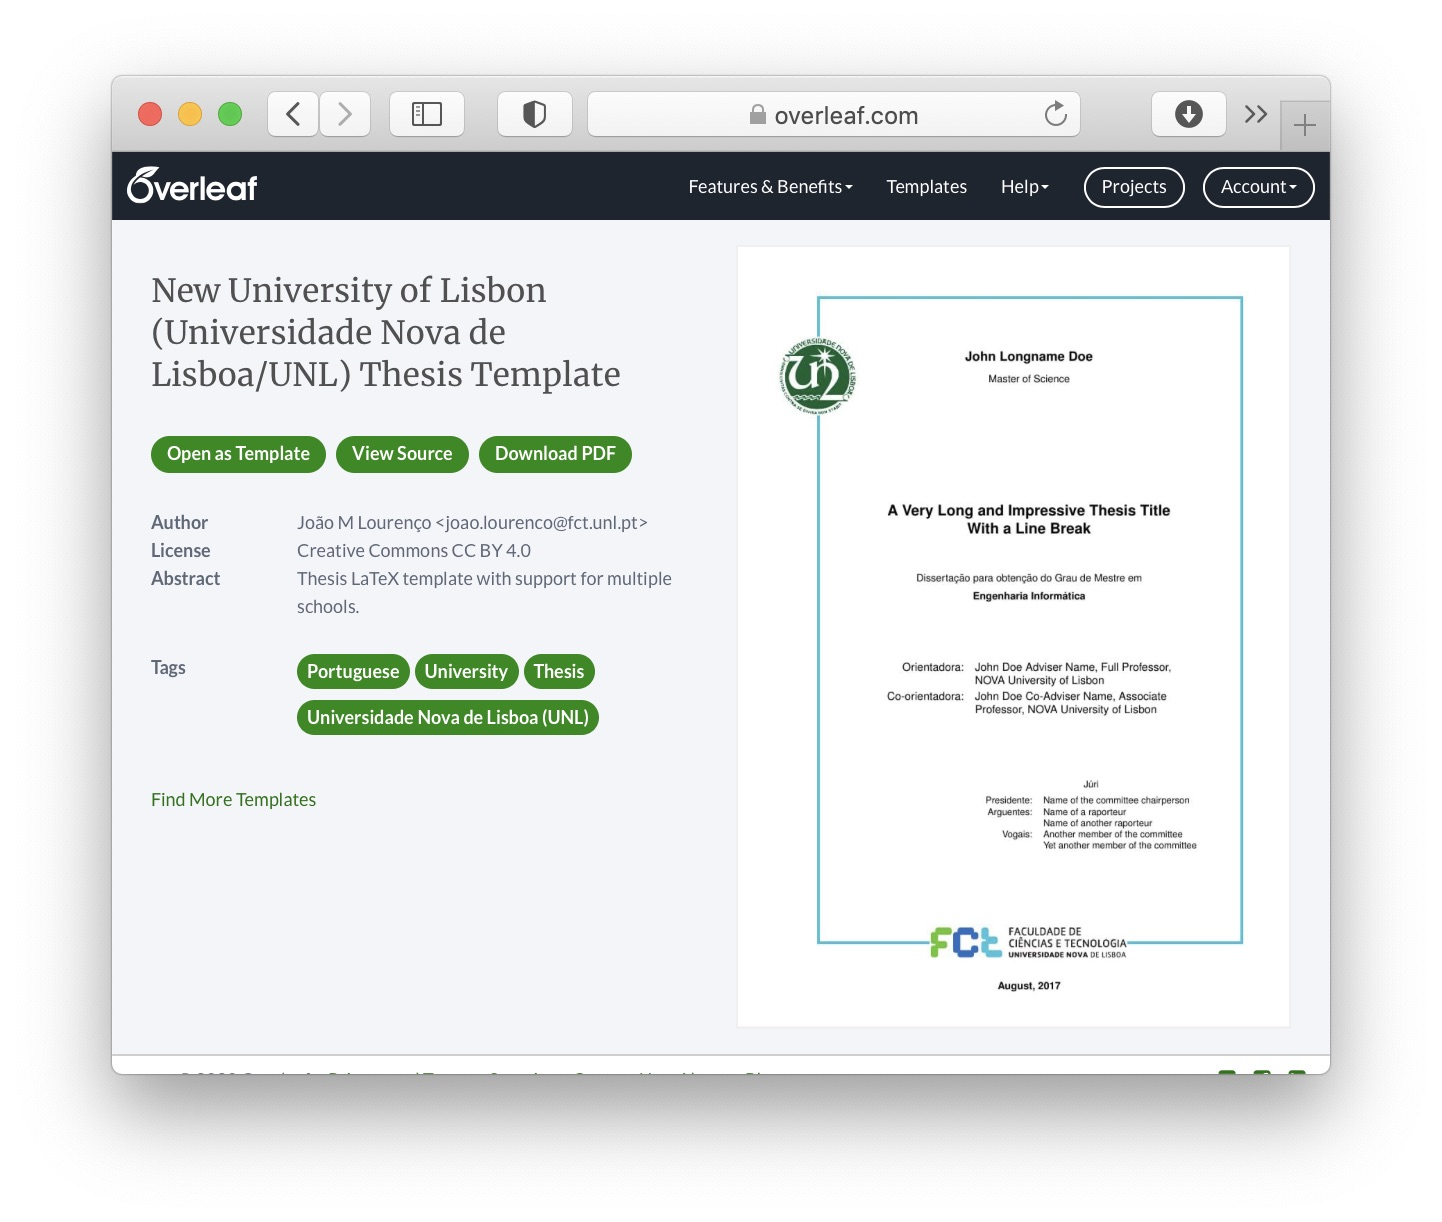
\includegraphics[width=\linewidth]{overleaf}%
\caption{NOVAthesis template in Overleaf.}
\label{fig:overleaf}
\end{wrapfigure}

If you do not have an account in \href{https://www.overleaf.com?r=f5160636&rm=d&rs=b}{Overleaf}, you must \href{https://www.overleaf.com?r=f5160636&rm=d&rs=b}{create one first}.

Once you have an account, please access the \gls{novathesis} template in \href{https://www.overleaf.com/latex/templates/new-university-of-lisbon-universidade-nova-de-lisboa-slash-unl-thesis-template/fwbztcrptjmg}{Overleaf} and select the green button \emph{Open as Template} (see \Autoref{fig:overleaf}).

\bgroup
  \itshape
  Please notice that the version currently available in Overleaf (v6.5.3) is slightly outdated (current version is v\novathesisversion). A new version will be submitted to Overleaf soon.  Until then, please:
  \begin{enumerate}
    \item Download the \href{https://github.com/joaomlourenco/novathesis/archive/master.zip}{latest version} from the GitHub repository as a Zip file.
    \item Login to your favorite LaTeX cloud service. I recommend \href{https://www.overleaf.com/?r=f5160636&rm=d&rs=b}{Overleaf} but there are alternatives (these instructions apply to Overleaf and you'll have to adapt for other providers).
    \item In the menu select: \texttt{New project} $\rightarrow$ \texttt{Upload project}.
    \item Upload the zip file.
    \item Select “template.tex” as the main file.
    \item Let Overleaf compile the document.
  \end{enumerate}
\egroup

\subsection{Using a Local \LaTeX\ Installation}
\label{sub:using_local_latex}


\begin{wrapfigure}{r}{0.3\linewidth}
\vspace*{-17ex}
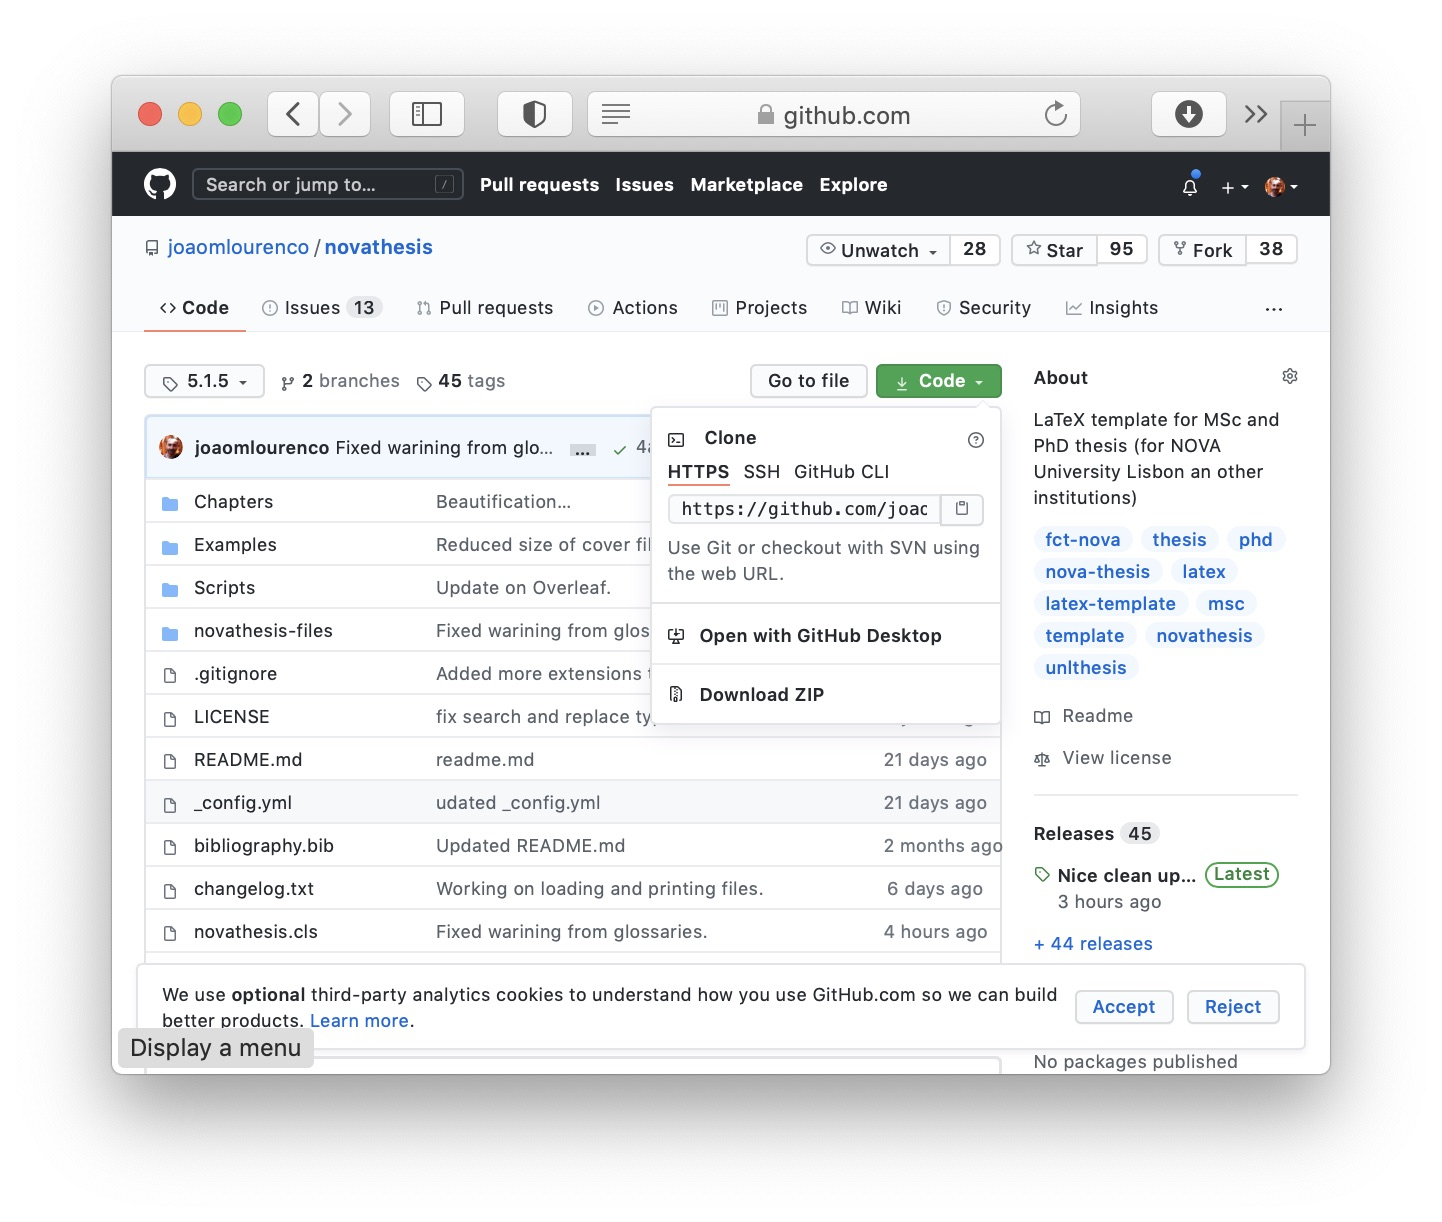
\includegraphics[width=\linewidth]{github}%
\caption{The NOVAthesis Project page in GitHub.}
\label{fig:github2}
\end{wrapfigure}

First of all, start by installing \LaTeX\ in your computer.  There are two main distributions, \href{https://miktex.org}{\MikTeX}\ and \href{https://www.tug.org/texlive/}{\TeXLive}, and both of them are available for the~3 most popular Operating Systems: Linux, macOS and Windows.

Be aware that a full installation of \MikTeX\ or \TeXLive\ will take near~5\,GB of hard disk space.  So, think twice before installing the full distribution.  See the \gls{novathesis} Wiki for the \href{https://github.com/joaomlourenco/novathesis/wiki/installing-latex#minimal-installation-in-any-of-the-systems-above}{list of packages required to compile the template}.

Once you have \LaTeX\ up and running, remember to install a good \LaTeX\ text editor.  I recommend you to take a look at  \href{https://tex.stackexchange.com/questions/339/latex-editors-ides}{this post} in the \url{tex.stackexchange.com} site.  If you want a quick and dirty recommendation, try \href{https://www.texstudio.org/}{TeXStudio}.

Now, you must access the \gls{novathesis} repository in \href{https://github.com/joaomlourenco/novathesis}{GitHub}, select the green button \emph{Code} and then \emph{download} (or \emph{clone}) the template.  You will always get the latest version of the template (currently v\novathesisversion\ from \novathesisdate).


\section{Getting Help}
\label{sec:getting_help}

No! You don't have to use this template to write your thesis.  You don't even have to use \LaTeX.  However, writing a thesis is serious stuff, and which tool you shall use to write it is not a decision to make lighthearted.

\LaTeX\ is hard enough by itself.  This template aims at making your life easier, but not easy. If you choose to use this template to write your thesis, you are very welcome.  However, don't expect me to provide you help with \LaTeX.  Look for help with your friends (you have some friends, don't you?), or search the web, or try even to read some book(s) on \LaTeX. In the end you will certainly find the experience rewarding.

When you come to the point of “\emph{How do I do this with \LaTeX?}”, remember…

\begin{enumerate}
  \item To check the \href{https://github.com/joaomlourenco/novathesis/wiki}{\gls{novathesis} wiki} and have some hope!  \emojiSmile
  \item Google is your best friend.
  \item Search the \href{https://github.com/joaomlourenco/novathesis/discussions}{GitHub Discussions page} for a question related to yours.  \emph{If and only if} you don't find one, then post your own question in English please!
  \item Search the \href{https://www.facebook.com/groups/novathesis}{NOVAtheis Facebook group} for a question related to yours.  \emph{If and only if} you don't find one, then post your own question in either Portuguese or English, at your preference.
\end{enumerate}

When you post your own question, remember to \textbf{always} state the \gls{novathesis} version number you are using and referring to.

\begin{center}  
  \fcolorbox{red}{gray!15}{\parbox{\textwidth}{\begin{center}\large\textbf{Please do not attempt to contact me directly (email, Messenger, etc)…\\I WILL NOT REPLY!}\end{center}}}
\end{center}
 

\subsection{Suggestions, Bugs and Feature Requests} % (fold)
\label{sub:suggestions_bugs_and_feature_requests}

\begin{description}
  \item[Help:] If you just need some help, see above \Autoref{sec:getting_help}.
  \item[Suggestion:] Do you have a suggestion/recommendation? Please add it to the wiki and help other users!
  \item[Bug:] Did you find a bug? Please open an issue. Thanks!
  \item[New Feature:] Would you like to request a new feature (or support of a new School)? Please open an issue. Thanks!

\end{description}



% subsection suggestions_bugs_and_feature_requests (end)




\section{Donors}
\label{sec:donations}

The \href{https://github.com/joaomlourenco/novathesis/wiki#donators}{list of \emph{Donnors}} is available in the \gls{novathesis} Project page.


\section{Disclaimer}
\label{sec:disclaimer}

Although the \gls{novathesis} template is endorsed by some Schools (e.g., \href{https://www.fct.unl.pt/estudante/informacao-academica/teses-e-dissertacoes}{linked from FCT-NOVA web site}), the \gls{novathesis} template \textbf{this not an official template} for any School.

The \gls{novathesis} template exists to make your life easier and we do our best to make it compliant to the supported ($+25$) Schools' regulations but, in the end of the line, you and only you are accountable for both the look and the contents of the document you submit as your thesis/dissertation.
